\section{Создание абстракций с помощью функций}
\subsection{Введение}

Компьютерная наука - это чрезвычайно обширная академическая дисциплина. Области глобально распределенных систем, искусственного интеллекта, робототехники, графики, безопасности, научных вычислений, компьютерной архитектуры и десятки развивающихся подобластей каждый год пополняются новыми методами и открытиями. Стремительный прогресс компьютерной науки не затронул практически ни одного аспекта человеческой жизни. Коммерция, коммуникация, наука, искусство, досуг и политика - все они были переосмыслены как компьютерные области.

Огромная производительность компьютерной науки возможна только потому, что она построена на элегантном и мощном наборе фундаментальных идей. Все вычисления начинаются с представления информации, определения логики ее обработки и разработки абстракций, которые управляют сложностью этой логики. Овладение этими основами потребует от нас понимания того, как именно компьютеры интерпретируют компьютерные программы и выполняют вычислительные процессы.

Эти фундаментальные идеи уже давно преподаются в Беркли по классическому учебнику Structure and Interpretation of Computer Programs (\url{https://mitpress.mit.edu/9780262510875/structure-and-interpretation-of-computer-programs/}) Гарольда Абельсона и Джеральда Джея Сассмана с Джули Сассман. Эти конспекты лекций в значительной степени заимствованы из этого учебника, который авторы любезно разрешили адаптировать и использовать повторно.

Начало нашего интеллектуального путешествия не требует пересмотра, и мы не должны ожидать, что он когда-либо понадобится.


\begin{quotation}
Мы собираемся изучить идею вычислительного процесса. Вычислительные процессы - это абстрактные существа, которые населяют компьютеры. По мере своего развития процессы манипулируют другими абстрактными вещами, называемыми данными. Развитие процесса направляется шаблоном правил, называемым программой. Люди создают программы для управления процессами. По сути, мы вызываем духов компьютера с помощью наших заклинаний.

Программы, которые мы используем для управления процессами, похожи на заклинания колдуна. Они тщательно составляются из символических выражений на заумных и эзотерических языках программирования, которые определяют задачи, которые мы хотим, чтобы выполняли наши процессы.

Вычислительный процесс в правильно работающем компьютере выполняет программы точно и аккуратно. Поэтому, подобно ученику колдуна, начинающие программисты должны научиться понимать и предвидеть последствия своих колдовских действий.

-Абельсон и Сассман, SICP (1993)
\end{quotation}

\subsubsection{Программирование на языке Python}
\begin{quotation}
Язык - это не столько то, что вы изучаете, сколько то, к чему вы приобщаетесь.

-Арика Окрент
\end{quotation}

Чтобы определить вычислительные процессы, нам нужен язык программирования, желательно такой, который смогут понять как многие люди, так и множество компьютеров. В этом курсе мы будем изучать язык Python.

Python - это широко распространенный язык программирования, который привлек энтузиастов из многих профессий: веб-программистов, игровых инженеров, ученых, академиков и даже разработчиков новых языков программирования. Изучая Python, вы присоединяетесь к сообществу разработчиков, насчитывающему миллион человек. Сообщества разработчиков - это чрезвычайно важные институты: их члены помогают друг другу решать проблемы, делятся своим кодом и опытом, а также коллективно разрабатывают программное обеспечение и инструменты. Благодаря своему вкладу преданные члены сообщества часто становятся знаменитостями и пользуются всеобщим уважением. Возможно, когда-нибудь и вы окажетесь в числе этих элитных Питонистов.

Сам язык Python - это продукт большого сообщества добровольцев (\url{https://www.python.org/community/}), которое гордится разнообразием своих участников. Язык был задуман и впервые реализован Гвидо ван Россумом (\url{https://en.wikipedia.org/wiki/Guido_van_Rossum}) в конце 1980-х годов. В первой главе его учебника по Python 3 (\url{https://docs.python.org/3/tutorial/appetite.html}) объясняется, почему Python так популярен среди множества существующих сегодня языков.

Python отлично подходит в качестве учебного языка, поскольку на протяжении всей своей истории разработчики Python подчеркивали возможность интерпретации кода Python человеком, что подкреплялось руководящими принципами Zen of Python (\url{https://peps.python.org/pep-0020/}) - красотой, простотой и читабельностью. Python особенно подходит для этого курса, потому что его широкий набор функций поддерживает множество различных стилей программирования, которые мы и будем изучать. Хотя не существует единого способа программирования на Python, есть набор соглашений, разделяемых сообществом разработчиков, которые облегчают процесс чтения, понимания и расширения существующих программ. Таким образом, сочетание гибкости и доступности Python позволяет студентам изучить множество парадигм программирования, а затем применить полученные знания в тысячах текущих проектов (\url{https://pypi.org}).

Эти материалы поддерживают дух SICP, знакомя с особенностями Python в сочетании с методами проектирования абстракций и строгой моделью вычислений. Кроме того, эти материалы содержат практическое введение в программирование на Python, включая некоторые расширенные возможности языка и наглядные примеры. Изучение Python будет происходить естественно по мере прохождения курса.

Однако Python - богатый язык с множеством функций и возможностей, и мы сознательно вводим их постепенно, по мере того как накладываем слой фундаментальных концепций компьютерной науки. Опытным студентам, которые хотят быстро вникнуть во все тонкости языка, мы рекомендуем прочитать книгу Марка Пилгрима "Погружение в Python 3" (\url{https://diveintopython3.net}), которая находится в свободном доступе в Интернете. Темы в этой книге существенно отличаются от тем данного курса, но книга содержит очень ценную практическую информацию по использованию языка Python. Предупреждаем: в отличие от этих материалов, "Погружение в Python 3" предполагает наличие значительного опыта программирования.

Лучший способ начать программировать на Python - это напрямую взаимодействовать с интерпретатором. В этом разделе описано, как установить Python 3, инициировать интерактивный сеанс с интерпретатором и начать программировать.

\subsubsection{Установка Python 3}
Как и любое другое замечательное программное обеспечение, Python имеет множество версий. В этом курсе будет использоваться самая последняя стабильная версия Python 3 (в настоящее время Python 3.2). На многих компьютерах уже установлены более старые версии Python, но они не подойдут для этого курса. Вы можете использовать любой компьютер для этого курса, но вам придется установить Python 3. Не волнуйтесь, Python бесплатен.

В книге Dive Into Python 3 есть подробные инструкции по установке для всех основных платформ (\url{https://diveintopython3.net/installing-python.html}). В этих инструкциях несколько раз упоминается Python 3.1, но вам лучше использовать Python 3.2 (хотя для данного курса различия незначительны). На всех учебных машинах кафедры EECS уже установлен Python 3.2.

\subsubsection{Интерактивные сессии}
В интерактивном сеансе Python вы вводите код Python после подсказки >>>. Интерпретатор Python читает и оценивает то, что вы вводите, выполняя ваши различные команды.

Существует несколько способов начать интерактивную сессию, и они отличаются по своим свойствам. Попробуйте их все, чтобы понять, что вам больше нравится. Все они используют один и тот же интерпретатор за кулисами.
\begin{itemize}
  \item Самый простой и распространенный способ - запустить приложение Python 3. Введите python3 в строке терминала (Mac/Unix/Linux) или откройте приложение Python 3 в Windows.
  \item Более удобное приложение для тех, кто изучает язык, называется IDLE 3 (IDLE3). IDLE раскрашивает ваш код (это называется подсветкой синтаксиса), выводит подсказки по использованию и указывает на источник некоторых ошибок. IDLE всегда поставляется в комплекте с Python, так что вы уже установили его.
  \item Редактор Emacs может запускать интерактивную сессию внутри одного из своих буферов. Хотя изучение Emacs несколько сложнее, это мощный и универсальный редактор для любого языка программирования. Прочитайте учебник 61A по Emacs, чтобы начать работу. Многие программисты, потратившие время на изучение Emacs, больше никогда не переходят на другие редакторы.
\end{itemize}

В любом случае, если вы видите строку интерпретатора Python, >>>, значит, вы успешно начали интерактивный сеанс. В этом примере показан пример взаимодействия с использованием интерпретатора и последующего ввода.

\begin{verbatim}
>>> 2 + 2
4
\end{verbatim}

Элементы управления: В каждом сеансе сохраняется история набранных вами символов. Чтобы получить доступ к этой истории, нажмите <Control>-P (предыдущий) и <Control>-N (следующий). Выход из сеанса <Control>-D удаляет эту историю.

\subsubsection{Первый пример}
\begin{quotation}
И, когда воображение создает

Формы вещей неведомых, и перо поэта

Превращает их в формы и дает воздушному ничто

Местное жилище и имя.

- Уильям Шекспир, "Сон в летнюю ночь".
\end{quotation}

Чтобы ознакомить вас с Python, мы начнем с примера, в котором используются несколько возможностей языка. В следующем разделе нам придется начать с нуля и создавать язык по частям. Воспринимайте этот раздел как предварительный просмотр будущих мощных возможностей.

В Python встроена поддержка широкого спектра распространенных операций программирования, таких как работа с текстом, отображение графики и общение через Интернет.

Оператор импорта

\begin{verbatim}
>>> from urllib.request import urlopen
\end{verbatim}

загружает функциональность для доступа к данным в Интернете. В частности, она делает доступной функцию urlopen, которая может получить доступ к содержимому по унифицированному локатору ресурсов (URL), который представляет собой местоположение чего-либо в Интернете.

Инструкции и выражения. Код Python состоит из инструкций и выражений. В общем случае компьютерные программы состоят из инструкций, направленных либо на:

\begin{enumerate}
  \item Вычислить некоторое значение
  \item Выполнить некоторое действие
\end{enumerate}

Инструкции обычно описывают действия. Когда интерпретатор Python выполняет инструкцию, он выполняет соответствующее действие. С другой стороны, выражения обычно описывают вычисления, которые дают значения. Когда Python вычисляет выражение, он вычисляет его значение. В этой главе мы познакомимся с несколькими типами инструкций и выражений.

Инструкция по присвоению

\begin{verbatim}
>>> shakespeare =
    urlopen('http://inst.eecs.berkeley.edu/~cs61a/fa11/shakespeare.txt')
\end{verbatim}

связывает имя shakespeare со значением выражения, которое следует за ним. Это выражение применяет функцию urlopen к URL-адресу, содержащему полный текст 37 пьес Уильяма Шекспира в одном текстовом документе.

Функции.
В функциях заключена логика, которая манипулирует данными.
Веб-адрес - это часть данных, а текст пьес Шекспира - другая.
Процесс, в результате которого первое приводит ко второму, может быть сложным, но мы можем применить этот процесс, используя лишь простое выражение, потому что эта сложность скрыта в функции.
Функции - основная тема этой главы.

Еще одна инструкция о присвоении

\begin{verbatim}
>>> words = set(shakespeare.read().decode().split())
\end{verbatim}

связывает имя words с набором всех уникальных слов, которые встречаются в пьесах Шекспира, - всего их 33 721. Цепочка команд чтения (read), декодирования (decode) и разбиения (split) оперирует с промежуточным вычислительным объектом: данные считываются из открытого URL, эти данные декодируются в текст, а текст разбивается на слова. Все эти слова помещаются в набор (set).

Объекты. Набор (set) - это тип объекта, который поддерживает такие операции с наборами, как вычисление пересечений и проверка принадлежности. Объект легко объединяет данные и логику, которая манипулирует этими данными, таким образом, чтобы скрыть сложность того и другого. Объекты являются основной темой главы 2.

Выражение

%\begin{lstlisting}
%
%\end{lstlisting}

\begin{verbatim}
>>> {w for w in words if len(w) >= 5 and w[::-1] in words}
{'madam', 'stink', 'leets', 'rever', 'drawer', 'stops', 'sessa',
'repaid', 'speed', 'redder', 'devil', 'minim', 'spots', 'asses',
'refer', 'lived', 'keels', 'diaper', 'sleek', 'steel', 'leper',
'level', 'deeps', 'repel', 'reward', 'knits'}
\end{verbatim}

это составное выражение, которое оценивает набор шекспировских слов, встречающихся как в прямом, так и в обратном порядке. Загадочная нотация w[::-1] перечисляет каждую букву в слове, но -1 говорит о том, что нужно двигаться назад (:: здесь означает, что позиции первого и последнего символов для перечисления заданы по умолчанию). Когда вы вводите выражение в интерактивной сессии, Python печатает его значение в следующей строке, как показано на рисунке.

Интерпретаторы. Вычисление составных выражений требует точной процедуры, которая интерпретирует код предсказуемым образом. Программа, реализующая такую процедуру, вычисляющая составные выражения и утверждения, называется интерпретатором. Проектирование и реализация интерпретаторов - основная тема главы 3.

По сравнению с другими компьютерными программами, интерпретаторы языков программирования уникальны своей общностью. Python не был разработан с расчетом на Шекспира или палиндромы. Однако его большая гибкость позволила нам обработать большой объем текста всего в нескольких строках кода.

В итоге мы увидим, что все эти основные понятия тесно связаны между собой: функции - это объекты, объекты - это функции, а интерпретаторы - это элементы тех и других. Однако четкое понимание каждой из этих концепций и их роли в организации кода имеет решающее значение для овладения искусством программирования.

\subsubsection{Практическое руководство: Ошибки}
Python ждет ваших команд. Вам рекомендуется экспериментировать с языком, даже если вы еще не знаете всего его словарного запаса и структуры. Однако будьте готовы к ошибкам. Хотя компьютеры невероятно быстры и гибки, они также чрезвычайно строги. Природа компьютеров описывается в вводном курсе Стэнфорда следующим образом

\begin{quotation}
Фундаментальное уравнение компьютеров таково: компьютер = мощный + глупый

Компьютеры очень мощные, они быстро обрабатывают большие объемы данных. Компьютеры могут выполнять

миллиарды операций в секунду, причем каждая операция довольно проста.

Компьютеры также потрясающе глупы и уязвимы. Операции, которые они могут выполнять, чрезвычайно строги, просты и механичны. Компьютеру не хватает чего-то похожего на настоящую проницательность... Он совсем не похож на HAL 9000 из фильмов. В любом случае, не стоит пугаться компьютера, как будто это какой-то мозг. Под ним скрывается очень механический аппарат.

Программирование - это когда человек использует свою настоящую интуицию, чтобы построить что-то полезное, сконструированное из этих маленьких, простых операций, которые может выполнять компьютер".

-Франциско Кай и Ник Парланте, Stanford CS101
\end{quotation}

Негибкость компьютеров сразу же станет очевидной, когда вы начнете экспериментировать с интерпретатором Python: даже самые незначительные изменения орфографии и форматирования приведут к неожиданным выводам и ошибкам.

Обучение распознаванию ошибок и диагностике причин неожиданных ошибок называется отладкой. Некоторые руководящие принципы отладки таковы:
\begin{enumerate}
  \item Тестирование пошагово: Каждая хорошо написанная программа состоит из небольших модульных компонентов, которые можно тестировать по отдельности. Тестируйте все, что вы пишете, как можно раньше, чтобы выявить ошибки на ранней стадии и обрести уверенность в своих компонентах.
  \item Изолировать ошибки: Ошибка в выводе составной программы, выражения или утверждения обычно может быть отнесена к определенному модульному компоненту. При попытке диагностировать проблему отследите ошибку до самого маленького фрагмента кода, прежде чем пытаться ее исправить.
  \item Проверка своих предположений: Интерпретаторы выполняют ваши инструкции в точности - не больше и не меньше. Их вывод становится неожиданным, когда поведение некоторого кода не соответствует тому, что считает (или предполагает) программист. Определите свои исходные предположения, а затем сосредоточьте усилия по отладке на проверке того, что ваши предположения действительно соответствуют действительности.
  \item Советоваться с другими: Вы не одиноки! Если вам непонятно сообщение об ошибке, спросите друга, преподавателя или поисковую систему. Если вы обнаружили ошибку, но не можете понять, как ее исправить, попросите кого-нибудь еще посмотреть. Многие ценные знания по программированию передаются в контексте командного решения проблем.
  \end{enumerate}

Поэтапное тестирование, модульное проектирование, точные предположения и работа в команде - темы, которые постоянно присутствуют в этом курсе. Надеемся, что они сохранятся и в вашей карьере в области компьютерных наук.

\subsection{Элементы программирования}
Язык программирования - это не просто средство, с помощью которого компьютер получает инструкции для выполнения задач. Язык также служит каркасом, в котором мы организуем наши идеи о вычислительных процессах. Программы служат для передачи этих идей членам сообщества программистов. Таким образом, программы должны быть написаны для того, чтобы их читали люди, и только потом для того, чтобы их выполняли машины.

Когда мы описываем язык, нам следует обратить особое внимание на средства, которые он предоставляет для объединения простых идей в более сложные. Каждый мощный язык имеет три таких механизма:
\begin{itemize}
  \item Примитивные выражения и операторы, представляющие собой простейшие строительные блоки, которые предоставляет язык
  \item средства комбинирования, с помощью которых сложные элементы создаются из более простых
  \item средства абстракции, с помощью которых составные элементы могут быть названы и управляться как отдельные единицы
  \end{itemize}

В программировании мы имеем дело с двумя видами элементов: функциями и данными. (Неформально данные - это материал, которым мы хотим манипулировать, а функции описывают правила манипулирования данными. Таким образом, любой мощный язык программирования должен уметь описывать примитивные данные и примитивные функции, а также иметь некоторые методы для комбинирования и абстрагирования как функций, так и данных.

\subsubsection{Выражения}
Поэкспериментировав с полноценным интерпретатором Python в предыдущем разделе, мы начинаем заново, методично осваивая язык Python элемент за элементом. Наберитесь терпения, если примеры покажутся вам упрощенными - скоро вас ждет более интересный материал.

Начнем с примитивных выражений. Одним из видов примитивных выражений является число. Точнее, выражение, которое вы вводите, состоит из цифр, обозначающих число по основанию 10.
\begin{verbatim}
  >>> 42
  42
  \end{verbatim}

Выражения, представляющие числа, могут быть объединены с математическими операторами, чтобы сформировать составное выражение, которое интерпретатор будет выполнять:
\begin{verbatim}
>>> -1 - -1
0
>>> 1/2 + 1/4 + 1/8 + 1/16 + 1/32 + 1/64 + 1/128
0.9921875
  \end{verbatim}

В этих математических выражениях используется инфиксная нотация, где оператор (например, +, -, * или /) находится между операндами (числами). В Python существует множество способов формирования составных выражений. Мы не будем пытаться перечислить их все сразу, а будем вводить новые формы выражений по мере продвижения, а также функции языка, которые они поддерживают.

\subsubsection{Вызов выражений}
Наиболее важным видом составного выражения является выражение вызова, которое применяет функцию к некоторым аргументам. Вспомните из алгебры, что математическое понятие функции - это отображение некоторых входных аргументов в выходное значение. Например, функция max сводит свои входящие значения к одному выходящему, которое является наибольшим из входящих. Способ, которым Python выражает применение функций, такой же, как и в обычной математике.
\begin{verbatim}
>>> max(7.5, 9.5)
9.5
  \end{verbatim}

Это выражение вызова имеет подвыражения: оператор - это выражение, стоящее перед круглыми скобками, в которых заключен список выражений-операндов, разделенных запятыми.
\begin{center}
  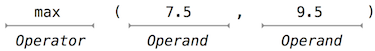
\includegraphics[scale=1]{call_expression.png}
\end{center}

Оператор задает функцию. Когда это выражение вызова вычисляется, мы говорим, что функция max вызывается с аргументами 7,5 и 9,5 и возвращает значение 9,5.

Порядок аргументов в выражении вызова имеет значение. Например, функция pow возводит первый аргумент в степень значения второго аргумента.
\begin{verbatim}
>>> pow(100, 2)
10000
>>> pow(2, 100)
1267650600228229401496703205376
  \end{verbatim}

Функциональная нотация имеет три основных преимущества перед математической конвенцией инфиксной нотации. Во-первых, функции могут принимать произвольное количество аргументов:
\begin{verbatim}
>>> max(1, -2, 3, -4)
3
  \end{verbatim}

Никакой двусмысленности возникнуть не может, поскольку имя функции всегда предшествует ее аргументам.

Во-вторых, обозначения функций легко распространяются на вложенные выражения, элементы которых сами являются составными выражениями. Во вложенных выражениях вызова, в отличие от составных инфиксных выражений, структура вложенности полностью явна в круглых скобках.
\begin{verbatim}
>>> max(min(1, -2), min(pow(3, 5), -4))
-2
  \end{verbatim}

Глубина такой вложенности и общая сложность выражений, которые может вычислить интерпретатор Python, в принципе не ограничена. Однако люди быстро запутываются в многоуровневой вложенности. Важная роль для вас как программиста - структурировать выражения так, чтобы они оставались интерпретируемыми для вас, ваших партнеров по программированию и других людей, которые могут читать ваши выражения в будущем.

В-третьих, математические обозначения имеют огромное разнообразие форм: умножение отображается между членами, экспоненты - как надстрочные знаки, деление - как горизонтальная полоска, а квадратный корень - как крыша с наклонной черепицей. Некоторые из этих обозначений очень трудно набирать! Однако вся эта сложность может быть унифицирована с помощью нотации выражений вызова. Хотя Python поддерживает общие математические операторы с использованием инфиксной нотации (например, + и -), любой оператор может быть выражен как функция с именем.

\subsubsection{Импорт библиотечных функций}
В Python определено очень большое количество функций, включая функции-операторы, упомянутые в предыдущем разделе, но по умолчанию их имена не доступны, чтобы избежать полного хаоса. Вместо этого язык организует функции и другие объекты, о которых он знает, в модули, которые вместе составляют библиотеку Python. Чтобы использовать эти элементы, нужно их импортировать. Например, модуль math предоставляет множество известных математических функций:
\begin{verbatim}
>>> from math import sqrt, exp
>>> sqrt(256)
16.0
>>> exp(1)
2.718281828459045
  \end{verbatim}

а модуль operator предоставляет доступ к функциям, соответствующим инфиксным операторам:
\begin{verbatim}
>>> from operator import add, sub, mul
>>> add(14, 28)
42
>>> sub(100, mul(7, add(8, 4)))
16
  \end{verbatim}

В операторе import указывается имя модуля (например, operator или math), а затем перечисляются именованные атрибуты этого модуля для импорта (например, sqrt или exp).

В документации по библиотеке Python 3 (\url{https://docs.python.org/3/library/index.html}) перечислены функции, определенные каждым модулем, например, модулем math (\url{https://docs.python.org/3/library/math.html}).
Однако эта документация написана для разработчиков, которые хорошо знают весь язык.
На данный момент вы можете обнаружить, что эксперименты с функцией расскажут вам больше о ее поведении, чем чтение документации.
По мере знакомства с языком и лексикой Python эта документация станет ценным справочным источником.

\subsubsection{Имена и окружения}
Важнейшим аспектом языка программирования являются средства, которые он предоставляет для использования имен для ссылки на исчисляемые объекты. Если значению присвоено имя, мы говорим, что имя связывается со значением.

В Python мы можем устанавливать новые связи с помощью оператора присваивания, который содержит имя слева от = и значение справа:
\begin{verbatim}
>>> radius = 10
>>> radius
10
>>> 2 * radius
20
  \end{verbatim}

Имена также связываются с помощью оператора import.
\begin{verbatim}
>>> from math import pi
>>> pi * 71 / 223
1.0002380197528042
  \end{verbatim}

Мы также можем присвоить несколько значений нескольким именам в одном операторе, где имена и выражения разделяются запятыми.
\begin{verbatim}
>>> area, circumference = pi * radius * radius, 2 * pi * radius
>>> area
314.1592653589793
>>> circumference
62.83185307179586
  \end{verbatim}

Символ = в Python (и многих других языках) называется оператором присваивания. Присваивание - это простейшее средство абстракции в Python, поскольку оно позволяет нам использовать простые имена для обозначения результатов сложных операций, таких как площадь, вычисленная выше. Таким образом, сложные программы строятся путем создания шаг за шагом вычислительных объектов все большей сложности.

Возможность связывания имен со значениями и последующего получения этих значений по имени означает, что интерпретатор должен содержать некую память, в которой хранятся имена, значения и связывания. Эта память называется окружением.

Имена также могут быть привязаны к функциям. Например, имя max связано с функцией max, которую мы использовали. Функции, в отличие от чисел, сложно вывести в виде текста, поэтому Python печатает идентифицирующее описание, когда его просят вывести функцию:
\begin{verbatim}
>>> max
<built-in function max>
  \end{verbatim}

Мы можем использовать операторы присваивания, чтобы дать новые имена существующим функциям.
\begin{verbatim}
>>> f = max
>>> f
<built-in function max>
>>> f(3, 4)
4
  \end{verbatim}

А последующие операторы присваивания могут перепривязать имя к новому значению.
\begin{verbatim}
>>> f = 2
>>> f
2
  \end{verbatim}

В Python имена, связанные с помощью присваивания, часто называют именами переменных, потому что они могут быть связаны с различными значениями в процессе выполнения программы.

\subsubsection{Вызов вложенных выражений}
Одна из наших целей в этой главе - выделить проблемы, связанные с процедурным мышлением.
В качестве примера рассмотрим, что при вычислении вложенных вызово выражений интерпретатор сам выполняет процедуру.

Чтобы вычислить вызов выражения, Python сделает следующее:
\begin{enumerate}
  \item Вычислит оператора и операнд подвыражений, затем
  \item Применит функцию, являющуюся значением оператора подвыражения, к аргументам, являющимся значениями операнда подвыражений.
\end{enumerate}

Даже эта простая процедура иллюстрирует некоторые важные моменты, касающиеся процессов в целом. Первый шаг диктует, что для выполнения процесса вычисления вызова выражения мы должны сначала вычислить другие выражения. Таким образом, процедура вычисления является рекурсивной по своей природе; то есть она включает, в качестве одного из своих шагов необходимость вызова самой себя.

Для примера вычисление
\begin{verbatim}
>>> mul(add(2, mul(4, 6)), add(3, 5))
208
\end{verbatim}

требует, чтобы эта процедура вычисления была применена четыре раза. Если мы нарисуем каждое выражение, которое мы вычисляем, то сможем представить себе иерархическую структуру этого процесса.
\begin{center}
  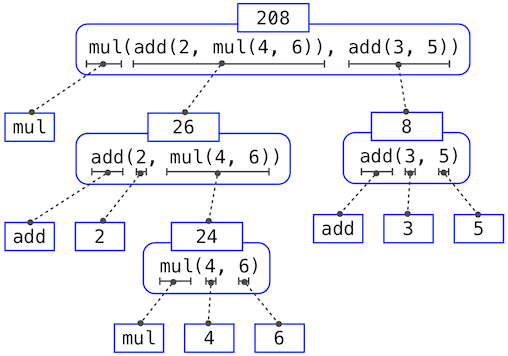
\includegraphics[scale=1]{expression_tree.png}
\end{center}

Эта иллюстрация называется деревом выражений. В компьютерной науке деревья растут сверху вниз. Объекты в каждой точке дерева называются узлами; в данном случае это выражения, сопряженные со своими значениями.

Для вычисления корня, полного выражения, необходимо сначала вычислить ветви, которые являются его подвыражениями. Листовые выражения (то есть узлы, не имеющие ответвлений) представляют собой либо функции, либо числа. Внутренние узлы состоят из двух частей: вызова выражения, к которому применяется наше правило вычисления, и результата этого выражения. Рассматривая вычисление в терминах этого дерева, мы можем представить, что значения операндов просачиваются вверх, начиная с конечных узлов и затем объединяясь на все более высоких уровнях.

Далее обратите внимание, что повторное применение первого шага приводит нас к тому, что нам нужно вычислять не вызов выражения, а примитивные выражения, такие как числа (например, 2) и имена (например, add). Мы позаботимся о примитивных случаях, указав, что
\begin{itemize}
  \item Цифра преобразуется как число, которое она обозначает,
  \item Имя вычисляется по значению, связанному с этим именем в текущей среде.
\end{itemize}

Обратите внимание на важную роль окружения в определении значения символов в выражениях. В Python бессмысленно говорить о значении такого выражения, как
\begin{verbatim}
>>> add(x, 1)
\end{verbatim}

не указывая никакой информации об окружении, которая могла бы обеспечить значение имени x (или даже имени add). Окружение обеспечивает контекст, в котором происходит вычисление, который играет важную роль в нашем понимании выполнения программы.

Этой процедуры вычисления недостаточно для оценки всего кода Python, только вызова выражения, чисел и имен. Например, она не обрабатывает операторы присваивания. Выполнение
\begin{verbatim}
>>> x = 3
\end{verbatim}

не возвращает значение и не вычисляет функцию по некоторым аргументам, поскольку цель присваивания - связать имя со значением. В общем случае инструкции не вычисляются, а выполняются; они не создают значение, а производят некоторое изменение. Для каждого типа инструкций или выражений существует своя процедура вычисления или выполнения, которую мы будем вводить постепенно, по мере продвижения вперед.

Обратите внимание: когда мы говорим, что " цифра преобразуется в число", на самом деле мы имеем в виду, что интерпретатор Python преобразует цифру в число. Именно интерпретатор наделяет язык программирования смыслом. Учитывая, что интерпретатор - это фиксированная программа, которая всегда ведет себя последовательно, можно сказать, что в контексте программ на Python цифры (и выражения) сами преобразуются в значения.

\subsubsection{Диаграммы функций}
Продолжая разрабатывать формальную модель вычисления, мы обнаружим, что диаграммы внутреннего состояния интерпретатора помогают нам отслеживать ход выполнения процедуры вычисления. Важной частью этих диаграмм является представление функции.

Чистые функции. Функции имеют некоторый вход (аргументы) и возвращают некоторый выход (результат их применения). Встроенную функцию
\begin{verbatim}
>>> abs(-2)
2
\end{verbatim}

можно изобразить в виде небольшой машины, которая принимает входные данные и производит выходные.
\begin{center}
  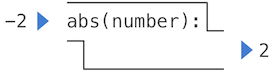
\includegraphics[scale=1]{function_abs.png}
\end{center}

Функция abs является чистой. Чистые функции обладают таким свойством, что их применение не имеет никаких эффектов, кроме возврата значения.

Нечистые функции. Помимо возврата значения, применение нечистой функции может генерировать побочные эффекты, которые вносят некоторые изменения в состояние интерпретатора или компьютера. Распространенным побочным эффектом является генерация дополнительного вывода, помимо возвращаемого значения, с помощью функции print.
\begin{verbatim}
>>> print(-2)
-2
>>> print(1, 2, 3)
1 2 3
\end{verbatim}

Хотя в этих примерах print и abs могут показаться похожими, они работают принципиально по-разному. Значение, которое возвращает print, - это всегда None, специальное значение Python, которое ничего не обозначает. Интерактивный интерпретатор Python не выводит значение None автоматически. В случае с print сама функция печатает вывод как побочный эффект от ее вызова.
\begin{center}
  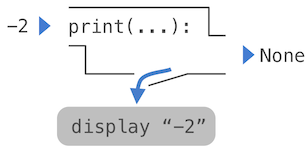
\includegraphics[scale=1]{function_print.png}
\end{center}

Вложенное выражение вызовов print подчеркивает нечистый характер функции.
\begin{verbatim}
>>> print(print(1), print(2))
1
2
None None
\end{verbatim}

Если этот вывод кажется вам неожиданным, нарисуйте дерево выражений, чтобы прояснить, почему выполнение этого выражения приводит к такому необычному результату.

Будьте осторожны с print! Тот факт, что она возвращает None, означает, что она не должна быть выражением в операторе присваивания.
\begin{verbatim}
>>> two = print(2)
2
>>> print(two)
None
\end{verbatim}

Сигнатуры. Функции различаются по количеству аргументов, которые они могут принимать. Чтобы отследить эти требования, мы рисуем каждую функцию таким образом, чтобы показать имя функции и имена ее аргументов. Функция abs принимает только один аргумент - число; указание большего или меньшего числа аргументов приведет к ошибке. Функция print может принимать произвольное количество аргументов, поэтому она отображается как print(...). Описание аргументов, которые может принимать функция, называется сигнатурой функции.

\subsection{Определение новых функций}
Мы выделили в Python некоторые элементы, которые должны присутствовать в любом мощном языке программирования:
\begin{enumerate}
  \item Числа и арифметические операции являюшиеся встроенными данными и функциями.
  \item Применение вложенных функций позволяющее комбинировать операции.
  \item Привязка имен к значениям обеспечивающее ограниченное средство абстракции.
\end{enumerate}
Теперь мы узнаем об определениях функций - более мощной технике абстракции, с помощью которой можно связать имя с составной операцией, на которую можно ссылаться как на элемент.

Начнем с того, что разберемся, как выразить идею "возведения в квадрат". Мы можем сказать: "Чтобы возвести что-то в квадрат, умножьте это на себя". На языке Python это выражается так
\begin{verbatim}
>>> def square(x):
        return mul(x, x)
\end{verbatim}

которая определяет новую функцию, получившую имя square. Эта пользовательская функция не встроена в интерпретатор. Она представляет собой составную операцию умножения чего-либо на само себя. Параметр x в этом определении называется формальным параметром, который дает имя тому, что нужно умножить. Определение создает эту пользовательскую функцию и связывает ее с именем square.

Определения функций состоят из оператора def, который указывает <имя> и список именованных <формальных параметров>, затем оператора return, называемого телом функции, который указывает <выражение возврата> функции, являющееся выражением, которое должно быть вычислено при каждом применении функции.
\begin{verbatim}
def <name>(<formal parameters>):
    return <return expression>
\end{verbatim}

Вторая строка должна быть с отступом! Согласно правилам, отступ должен состоять из четырех пробелов, а не из табуляции. Выражение return не вычисляется сразу; оно хранится как часть только что определенной функции и вычисляется только при ее применении. (Вскоре мы увидим, что область отступа может занимать несколько строк).

После определения квадрата мы можем применить его с помощью выражения вызова:
\begin{verbatim}
>>> square(21)
441
>>> square(add(2, 5))
49
>>> square(square(3))
81
\end{verbatim}

Мы также можем использовать квадрат в качестве строительного блока для определения других функций.
Например, мы можем легко определить функцию sum\_squares, которая, принимая в качестве аргументов любые два числа, возвращает сумму их квадратов:
\begin{verbatim}
>>> def sum_squares(x, y):
        return add(square(x), square(y))
>>> sum_squares(3, 4)
25
\end{verbatim}

Определяемые пользователем функции используются точно так же, как и встроенные.
Действительно, из определения sum\_squares нельзя понять, является ли square встроенной в интерпретатор, импортированной из модуля или определенной пользователем.

\subsubsection{Окружения}
Наше подмножество Python стало настолько сложным, что смысл программ становится неочевидным. Что делать, если формальный параметр имеет то же имя, что и встроенная функция? Могут ли две функции иметь общие имена без путаницы? Чтобы решить эти вопросы, мы должны описать окружения более подробно.

Окружение, в котором вычисляется выражение, состоит из последовательности фреймов, изображенных в виде блоков. Каждый фрейм содержит привязки, которые связывают имя с соответствующим значением. Существует один глобальный фрейм, который содержит привязки имен для всех встроенных функций (показаны только abs и max). Мы обозначаем глобальный фрейм символом глобуса.
\begin{center}
  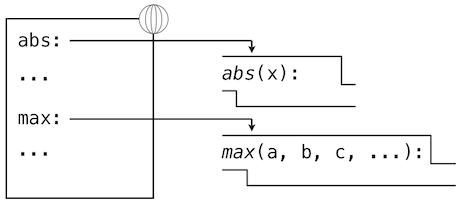
\includegraphics[scale=1]{global_frame.png}
\end{center}

Операторы присваивания и импорта добавляют записи в первый фрейм текущего окружения. Пока что наше окружение состоит только из глобального фрейма.
\begin{verbatim}
>>> from math import pi
>>> tau = 2 * pi
\end{verbatim}

\begin{center}
  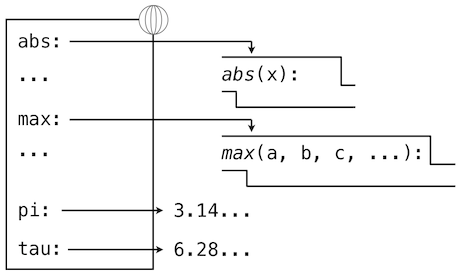
\includegraphics[scale=1]{global_frame_assignment.png}
\end{center}

Оператор def также привязывает имя к функции, созданной с помощью определения. Ниже показана результирующая среда после определения square:
\begin{center}
  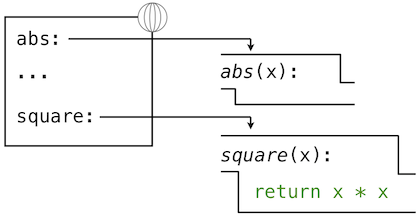
\includegraphics[scale=1]{global_frame_def.png}
\end{center}

Эти диаграммы окружения показывают привязки текущего окружения, а также значения (которые не являются частью какого-либо фрейма), к которым привязаны имена. Обратите внимание, что имя функции повторяется, один раз во фрейме и один раз как часть самой функции. Это повторение намеренное: множество различных имен может ссылаться на одну и ту же функцию, но сама функция имеет только одно собственное имя. Однако поиск значения имени в среде позволяет проверить только привязку к имени. Внутреннее имя функции не играет никакой роли при поиске имен. В примере, который мы рассматривали ранее,
\begin{verbatim}
>>> f = max
>>> f
<built-in function max>
\end{verbatim}

Имя max - это внутреннее имя функции, и именно его вы видите в качестве значения для f. Кроме того, оба имени - max и f - привязаны к одной и той же функции в глобальном окружении.

По мере внедрения дополнительных возможностей Python нам придется расширять эти диаграммы. Каждый раз, когда мы будем это делать, мы будем перечислять новые возможности, которые могут выразить наши диаграммы.

Новые возможности среды: Назначение и определение пользовательских функций.

\subsubsection{Вызов функций определенных пользователем}

Для выполнения вызова выражения, оператор которого определяет пользовательскую функцию, интерпретатор Python использует процесс, аналогичный тому, который применяется для вычисления выражений встроенных операторов функций.
То есть интерпретатор вычисляет выражения-операнды, а затем применяет именованную функцию к полученным аргументам.

При применении пользовательской функции создается второй локальный фрейм, который доступен только этой функции. Для применения пользовательской функции к некоторым аргументам:
\begin{enumerate}
  \item Привязываются аргументы к именам формальных параметров функции в новом локальном фрейме.
  \item Вычисляется тело функции в окружении, расположенном начиная с этого фрейма и заканчивая глобальным фреймом.
\end{enumerate}
Среда, в которой вычисляется тело функции, состоит из двух фреймов: сначала локальный фрейм, содержащий привязки аргументов, затем глобальный фрейм, содержащий все остальное. Каждый экземпляр функционального приложения имеет свой собственный независимый локальный фрейм.
\begin{center}
  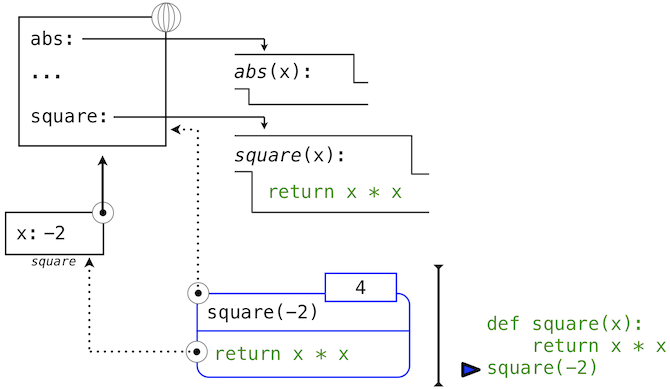
\includegraphics[scale=1]{evaluate_square.png}
\end{center}

Этот рисунок включает в себя два различных аспекта интерпретатора Python: текущее окружение и часть дерева выражений, связанного с текущей вычисляемой строкой кода.
Мы изобразили вычисление вызываемого выражения, содержащего определяемую пользователем функцию (синим цветом), в виде закругленного прямоугольника, состоящего из двух частей.
Пунктирные стрелки указывают, какое окружение используется для вычисления выражения в каждой части.
\begin{itemize}
  \item В верхней половине показано вызыв выражения, которое вычисляется. Этот вызов выражения не является внутренним для какой-либо функции, поэтому оно вычисляется в глобальном окружении. Таким образом, любые имена внутри него (например, square) будут искаться в глобальном фрейме.
  \item В нижней половине показано тело функции square. Ее возвращаемое выражение вычисляется в новом окружении, введенном шагом 1 выше, которое связывает имя формального параметра square x со значением его аргумента -2.
\end{itemize}

Порядок фреймов в окружении влияет на значение, возвращаемое при поиске имени в выражении. Ранее мы говорили, что имя вычисляется по значению, связанному с этим именем в текущем окружении. Теперь мы можем быть более точными:
\begin{itemize}
  \item Имя вычисляется по значению, связанному с этим именем в самом раннем кадре текущего окружения, в котором это имя обнаружено.
\end{itemize}

Наша концептуальная схема окружений, имен и функций представляет собой модель вычисления; хотя некоторые механические детали еще не определены (например, как реализуется связывание), наша модель точно и правильно описывает, как интерпретатор оценивает выражения вызова. В главе 3 мы увидим, как эта модель может служить образцом для реализации рабочего интерпретатора для языка программирования.

Новая возможность среды: Функция прикладного использования (Function application).

\subsubsection{Пример вызова функции определенной пользователем}
Давайте снова рассмотрим наши два простых определения:
\begin{verbatim}
>>> from operator import add, mul
>>> def square(x):
        return mul(x, x)
>>> def sum_squares(x, y):
        return add(square(x), square(y))
\end{verbatim}

\begin{center}
  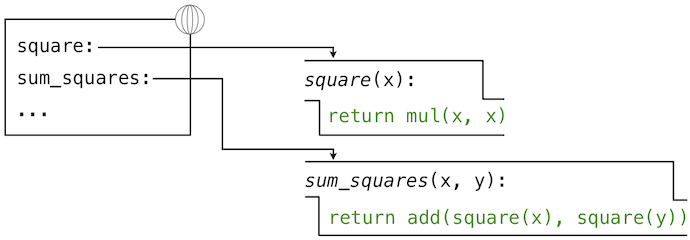
\includegraphics[scale=1]{evaluate_sum_squares_0.png}
\end{center}

И процесс, который вычисляет следующий вызов выражения:
\begin{verbatim}
>>> sum_squares(5, 12)
169
\end{verbatim}

Сначала Python вычисляет имя sum\_squares, которое привязано к пользовательской функции в глобальном фрейме.
Примитивные числовые выражения 5 и 12 преобразуются в числа, которые они представляют.

Затем Python применяет sum\_squares, что вводит локальный фрейм, связывающий x с 5, а y с 12.
\begin{center}
  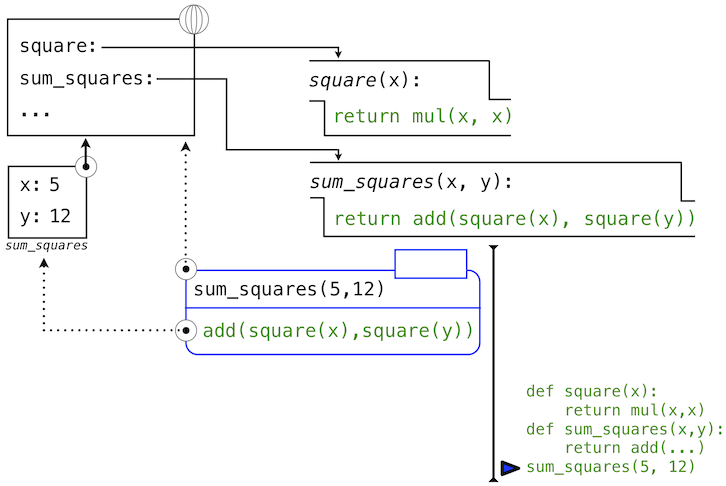
\includegraphics[scale=1]{evaluate_sum_squares_1.png}
\end{center}

На этой диаграмме локальный фрейм указывает на своего преемника - глобальный фрейм.
Все локальные фреймы должны указывать на предшественника, и эти связи определяют последовательность фреймов, которая является текущим окружением.

Тело sum\_squares содержит это выражение вызова:
\begin{center}
  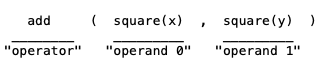
\includegraphics[scale=0.6]{sch_0.png}
\end{center}

Все три подвыражения вычисляются в текущем окружении, которое начинается с фрейма с меткой sum\_squares.
Оператор подвыражения add - это имя, найденное в глобальном фрейме, связанное со встроенной функцией сложения.
Два операнда подвыражения должны быть поочередно вычислены, прежде чем будет применено сложение.
Оба операнда вычисляются в текущем окружении, начиная с фрейма с меткой sum\_squares.
В следующих диаграммах окружения мы будем называть этот фрейм A и заменять стрелки, указывающие на этот фрейм, меткой A.

В операнде 0 square обозначает пользовательскую функцию в глобальном фрейме, а x - число 5 в локальном фрейме.
Python применяет square к 5, вводя еще один локальный фрейм, который связывает x с 5.
\begin{center}
  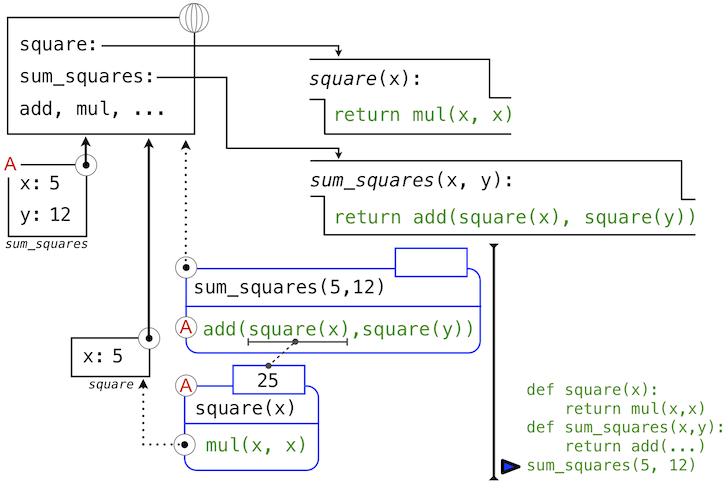
\includegraphics[scale=1]{evaluate_sum_squares_2.png}
\end{center}

Используя этот локальный фрейм, тело выражения mul(x, x) вычисляется как 25.

Теперь наша процедура вычисления переходит к операнду 1, для которому y соответствует число 12.
Python снова оценивает тело square, на этот раз вводя еще один локальный фрейм окружения, который связывает x с 12. Таким образом, операнд 1 получит значение 144.
\begin{center}
  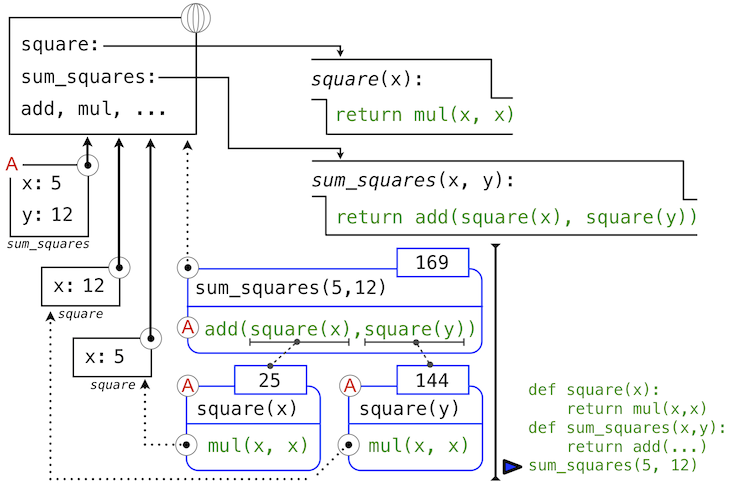
\includegraphics[scale=1]{evaluate_sum_squares_3.png}
\end{center}

Наконец, применение сложения к аргументам 25 и 144 дает окончательное значение для тела sum\_squares: 169.

Этот пример, несмотря на свою сложность, служит иллюстрацией многих фундаментальных идей, которые мы обсуждали до этого момента.
Имена привязаны к значениям, которые распределены по многим локальным фреймам, предшествующим одному глобальному фрейму, содержащему общие имена.
Выражения имеют древовидную структуру, и окружение должно дополняться каждый раз, когда подвыражение содержит вызов определенной пользователем функции.

Весь этот механизм существует для того, чтобы гарантировать, что имена преобразуются в правильные значения в правильных точках дерева выражений.
Этот пример иллюстрирует, почему наша модель требует той сложности, которую мы ввели.
Все три локальных фрейма содержат привязку для имени x, но это имя связано с разными значениями в разных фреймах. Локальные фреймы хранят эти имена отдельно.

\subsubsection{Локальные имена}
Одна из деталей реализации функции, которая не должна влиять на ее поведение, - это выбор исполнителем имен для формальных параметров функции. Таким образом, следующие функции должны обеспечивать одинаковое поведение:
\begin{verbatim}
>>> def square(x):
        return mul(x, x)
>>> def square(y):
        return mul(y, y)
\end{verbatim}

Этот принцип - что смысл функции должен быть независим от имен параметров, выбранных ее автором, - имеет важные последствия для языков программирования.
Самое простое следствие заключается в том, что имена параметров функции должны оставаться привязанными к телу функции.

Если бы параметры не были привязаны к телу соответствующих функций, то параметр x в square можно было бы спутать с параметром x в sum_squares.
Критически важно, что это не так: привязки для x в разных локальных фреймах не связаны. Наша модель вычислений тщательно продумана, чтобы обеспечить эту независимость.

Мы говорим, что область действия локального имени ограничена телом определяемой пользователем функции, которая его определяет.
Когда имя больше недоступно, оно выходит из области видимости. Такое поведение области видимости не является новым фактом в нашей модели; это следствие того, как работают среды.

